\documentclass[letterpaper,10pt,twocolumn]{article}
\usepackage{usenix}

\usepackage{footmisc}
%\usepackage[T1]{fontenc}
%\usepackage{fontspec}
%\setmainfont{Times New Roman}
\usepackage{times}
\usepackage{xcolor}
\usepackage{xspace}
\usepackage{type1cm}
\usepackage{boxedminipage}
\usepackage{pifont}
\usepackage{pseudocode}
\usepackage{multirow}
\usepackage{tabularx}
\usepackage{caption}
\usepackage{subcaption}
\usepackage{graphicx}

\definecolor{MyDarkBlue}{rgb}{0,0.08,0.45}
\usepackage[pdftex]{hyperref}
\hypersetup{
  colorlinks,%
  citecolor=MyDarkBlue,%
  filecolor=MyDarkBlue,%
  linkcolor=MyDarkBlue,%
  urlcolor=MyDarkBlue
}
\usepackage{fixltx2e}
\usepackage{textgreek}
\usepackage[sort]{cite}

% ---------------- Notes: -----------------------

\newcommand{\tbd}[1]{{\bf [[TBD: {#1}]]}}
\newcommand{\eat}[1]{}

\newcommand{\num}[1]{{\color{red}\bf {#1}}}

%\newcommand{\colin}[1]{{\color{red}\bf CS: {#1}}}
%\newcommand{\scott}[1]{{\color{purple}\bf SS: {#1}}}

\newcommand{\colin}[1]{}
\newcommand{\scott}[1]{}

\sloppy

\title{(Hypothesis): Caching Doesn't Improve Web Page Performance (Much)}

\author{
\rm Jamshed Vesuna$^\dagger$ \hspace{-7mm}
\and \rm Colin Scott$^\dagger$ \hspace{-7mm}
\and \rm Michael Buettner$^\diamond$ \hspace{-7mm}
\and \rm Michael Piatek$^\diamond$ \hspace{-7mm}
\and \rm Arvind Krishnamurthy$^\star$ \hspace{-7mm}
\and \rm Scott Shenker$^\dagger$ \\
\and {\begin{tabular}{ccc}$^\dagger$UC Berkeley \& ICSI & $^\diamond$Google &
$^\star$University of Washington\end{tabular}}}
% Also: \ddager, ^\text{\o}

\begin{document}
   \date{}
   \maketitle
   \thispagestyle{empty}

\section{Introduction}
\label{sec:intro}
\label{intro}
%With the increase in mobile Internet traffic, there is a larger emphasis on methods of improving web performance for mobile devices.
Web caching is widely used to reduce network link utilization, decrease server load and data usage, improve reliability for origin web servers, and improve latency for end hosts.
Here, we focus exclusively on web caching's effect on latency, as measured by web page load time.

Flywheel~\cite{flywheel}, Google's HTTP proxy for mobile devices, increased
its overall cache hit ratio from 22\% to 32\%, yet observed only a 1--2\% reduction in page load time in the median case.
Here we seek to gain a deeper understanding of why improved caching had such a negligible effect on performance.

% Can we remove this first sentence?
%Our contributions are as follows.
We present a methodology
% Commenting this out because they don't know what WPR and Telemetry are yet.
%based on Web Page Replay~\cite{wpr} and Telemetry~\cite{telemetry}
for evaluating the performance impact of web caching for hypothetical levels of cache hit ratios, in a controlled environment. We use this methodology to compare the effects of partial (hit ratio of 20\% to 30\%) and
perfect caching (hit ratio of 100\%) versus no caching for a set of 400 Alexa web pages~\cite{alexa} on both a mobile device and a desktop browser.

We demonstrate that by increasing the cache hit ratio from 20\% to 30\%, there is only a meager 1\% reduction in mobile web page load time.
Further, we show that with perfect caching, desktop page load times are improved notably by 34\% compared to no caching, but mobile page load times only improve by 13\% in the median case.
We finally show that CPU speed is the key resource bottleneck preventing mobile devices from benefiting significantly from web caching.

Our results suggest that the common wisdom that web caching is a crucial part of web performance optimization may not hold for mobile clients. Content providers may want to reconsider where they focus their efforts, especially as the volume of mobile traffic begins to overtake desktop traffic.

% TODO(cs): attempt to argue that others, besides the Flywheel authors, also
% suffer from the same misconception about web caching's potential benefits?


\section{Results}
\label{sec:results}
Here, we demonstrate empirical performance results we have found with our
apparatus. We also attempt to highlight the underlying effects that determine
our results.

\subsection{Workload Characteristics}
We first note several key characteristics of our data corpus:

\textbf{Data Set}. We selected a random subset of 400 of the Alexa top 2000 URLs~\cite{alexa} and loaded their root URL (`/').
% \textbf{Cache Hit Ratio}. We experiment with two settings of cache hit ratio. To show an upper bound on how much caching can help, we evaluate the effect of a perfect (100\%) cache. We also seek to reproduce the result from Flywheel~\cite{flywheel}, by showing the difference between 20\% and 30\% cache hit ratio.
% %In their NSDI paper, Google reported that increasing the cache hit ratio by more than 50\% only increased mobile PLT by 1-2\%. Here, we seek to capture an upper bound on caching's effect on PLT. 

\textbf{Fraction of Cacheable Bytes}. Over 90\% of web pages in our workload have more than 90\% of their total bytes marked as cacheable, as shown in Figure~\ref{fig:cacheable_bytes_linear}. %This gives the initial impression that perfect caching should have a significant effect on web performance.
%Web pages generally make high use of caching between origin servers and users.

\textbf{Total Bytes}. Figure~\ref{fig:total_bytes_linear} shows the spread of web page sizes in our data set. While 95\% of web pages are under 6.8 MB, the median web page size is less than 1.2 MB.

\textbf{Initial Network Delays}. Across all requests/response pairs, the median delay between sending the request and receiving the first response byte was 50ms, with a mean of 151.17ms and standard deviation of 403.77ms.
%Initial network delays may play a role in determining the final results of our caching analysis. 
% TODO(cs): we should include this next sentence?!
%As such, we experimented with inflating all network delays by a fixed amount (100ms) to emulate what clients in an emerging market might observe. We found that the mobile results of our caching analysis were changed by 3\% in the median case (See Figure~\ref{fig:inflated_delays}).
%\arvind{this is to the original website right?  the "LAN" is confusing.}

\textbf{User Agent}. Many web pages are now optimized for mobile devices. Web
servers inspect the user agents (UA) of incoming HTTP(S) requests to deliver
customized content to the client depending on their device size and
computational resources. We ran all of our experiments twice: once where the
browsers (both desktop and mobile) advertised a mobile UA, and once where the
browsers advertised a desktop UA. We found that the differences in the results
were comparable. Here, we show only the desktop UA results to make our graphs more readable.
%\arvind{shouldn't it be that the mobile device should use mobile UA and the desktop one should use the desktop UA? the fact that the differences - as opposed to the actual values - are comparable is interesting.} \jamshed{Add slight anecdotal evidence}

\subsection{Performance Results}

As we saw in Figure~\ref{fig:cacheable_bytes_linear}, most pages are composed of a significant number of cacheable bytes. This would seem to suggest that increasing the cache hit ratio should yield a significant improvement in web performance for the end user~\cite{kroeger1997exploring}.

\textbf{Caching Doesn't Significantly Reduce Mobile PLT}.
Similar to Flywheel's result~\cite{flywheel}, we find that increasing the cache hit ratio of a web page does not significantly decrease the user's overall latency on a mobile device.
In fact, with a perfect cache, a mobile device gains only a 13\% PLT reduction in the median case, while its desktop counterpart sees a  PLT reduction of 34\% (see Figure~\ref{fig:percent_reduction_linear}).

Additionally, we emulated partial caches with 20\% and 30\% hit ratios. As shown in Figure~\ref{fig:partial_cache_linear}, we found that increasing the hit ratio by 10 percentage points had negligible effects on mobile page load time. Consistent with Flywheel's NSDI paper, there was only a 1\% reduction in PLT in the median case.

Figure~\ref{fig:ratio_linear_comparison} illustrates how the impact of caching on PLT is limited:
for each 10 percentage point increase in cache hit ratio, there is only a 1 percentage point decrease in mobile page load time.
That is, there is a sharply diminishing marginal performance gain for every additional byte that is cached.
This experiemental evidence supports our model:
the fraction of cacheable bytes on the critical path ($K$) is significantly smaller than the fraction of cacheable byes \textbf{not} on the critical path.

Further, Figure~\ref{fig:plt_cpu_comparison} empirically shows that as CPU speed decreases, the computational time spent processing a web page ($C$) dominates overall PLT, while for faster CPUs, network delays account for most of the PLT ($ C << N $).

\begin{figure}[t]
    %\hspace{-10pt}
    \figuretitle{Ratio of Fraction Cacheable Bytes to PLT}
    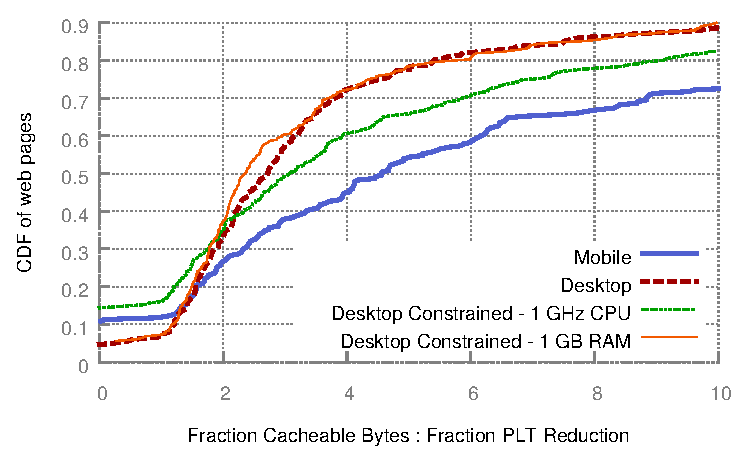
\includegraphics[width=3in]{../graphs/ratio_bytes_to_reduction/ratio_linear_comparison.pdf}
    \caption[]{\label{fig:ratio_linear_comparison}As the percentage of cacheable bytes in a web page increases, the reduction in page load time due to caching increases. However, for each additional percentage cached, there is less than a percentage reduction in page load time.}
\end{figure}
\subsection{Isolating the Difference Between Mobile and Desktop}

% Discuss resource constraints, CPU
We find that the main cause of discrepancy is due to the large difference of CPU speed between desktops and mobile devices. 
We measured this effect by running the same experiment as before, but in virtual machines that were constrained by different resources (using VirtualBox to either set a limit on memory usage or emulate a slower CPU clock speed).
A typical mobile device in the global market today has a 1 GHz processor and 1 GB of RAM~\cite{mobile-stats}. In order to emulate these conditions and isolate computational resources, we restricted one virtual machine to a 1 GHz processor with 6 GB of memory, and another to a 3.2 GHz processor with 1 GB of RAM.

%\colin{Need to also say how much memory/CPU it had, even if if you're focusing on CPU/memory}
In Figure~\ref{fig:percent_reduction_linear}, `Desktop Constrained - 1 GHz CPU' is closely aligned with the results for `Mobile' (our tablet), while `Desktop Constrained - 1 GB RAM' is more closely aligned with the `Desktop' results.
This suggest that CPU is the key difference between caching's effects for mobile and desktop.
In fact, as we throttle CPU constraints, perfect caching has noticeably smaller effects on PLT (See Figure~\ref{fig:plt_cpu_comparison}). Similarly, page load times are generally higher on devices with CPU constraints as seen in Figure~\ref{fig:plt_differences}.

%\colin{Can cut this if we need space}
Consistent with the results found in WProf~\cite{wang2013demystifying}, our results show that reduction in PLT is not proportional to number of bytes cached. We conjecture that the reason mobile performs worse than desktop is precisely because a constrained CPU changes the critical path (when compared to desktop), causing a smaller fraction of the critical path to be network-bound. 
%We hypothesize that the delays of objects on the critical path are also elongated by a constrained CPU.
%These factors contribute to a longer critical path that is prone to the benefits of caching.
%\arvind{above discussion is not clear; and it is probably the most critical observation that we need to communicate precisely}


\subsection{Data Validation}
\label{subsec:validation}
We made several efforts to sanity check the validity our results~\cite{sanity-checks}. To mitigate non-determinism, we compared the status codes of all objects loaded in the browser from both original and perfect/partial cache benchmarks. We filtered out about 9\% of web pages in our 400 URL data set in cases where there were a high number of 404 error codes due to non-deterministic requests without responses in the WPR archive. It is worth noting that the figures we present show only these 91\% of web pages that passed this filter.

As the ratio of cached to non-cached bytes increases in a web page, we expect page load time to be less than or equal to that of its non-cached counterpart. As seen in Figure~\ref{fig:ratio_linear_comparison}, there is a positive correlation between the fraction of cached bytes and the reduction in PLT, albeit asymptotic.
However, due to variance in PLT (discussed in \ref{known_limitations}), we see that a fraction of web pages can perform worse when cached, as seen by points to the left of \texttt{X = 0} in Figure~\ref{fig:percent_reduction_linear}.



\begin{figure}[t]
    %\hspace*{-0.11in}
    \figuretitle{CPU Comparison of PLT Reduction}
    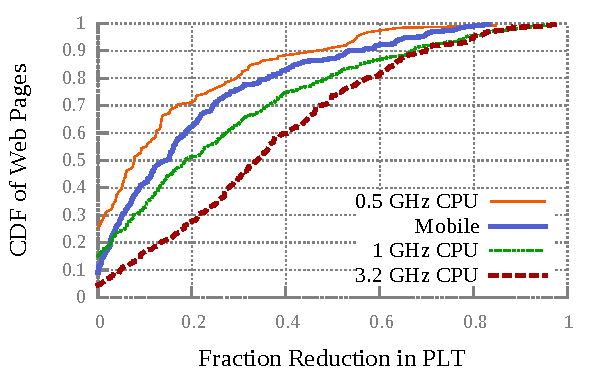
\includegraphics[width=3in]{../graphs/percent_plt_reduction/percent_reduction_linear_CPU_comparison.pdf}
    \caption[]{\label{fig:plt_cpu_comparison}Slower CPU speeds curtail the efficacy of caching to reduce page load time.}
\end{figure}


\section{Related Work}
\label{sec:related_work}
%Due to the burgeoning interest in web page speed, there has been a recent rise of network caching literature, tools, and companies.

% TODO(cs): explain that in the NSDI'15 slides, we presented a simple critical
% path model, and
% conjectured that objects on the critical path are often not in cache
% (cacheable). However, we didn't have any evidence for this.

Several papers have analyzed web page performance, the effects of caching, and the relationship between CPU speeds and page load time.
% As far as we know, we are the first to jointly isolate all of these factors. % this enables us to easily dissect the effects that caching has on mobile devices.

\textbf{WProf}. Wang et al.~\cite{wang2013demystifying} is the closest research to ours. As we discussed in ~\S\ref{sec:background}, the experiments WProf ran for their Figure 11 show that objects on the critical path are often not cached; and the experiments they ran for their
Figure 13 implies that decreasing CPU speed causes computational delays to comprise a larger fraction of the critical path.

We extend their research along several dimensions.
We develop a model that allows us to predict PLT for a given cache hit ratio. We show that limited RAM does not increase computational delays, though slow CPUs do. We also empirically measure (rather than statically compute, as WProf does) PLTs using a tablet device, and using CPU-constrained virtual machines, over a larger data set (400 URLs, vs. {\footnotesize$\sim$}50 URLs).
Lastly, we extend WProf's cacheability analysis to show that the
marginal returns from caching sharply diminish.

% WProf found that:
%   - Fig 11a & 11b, taken together, seem to imply that objects on the critical
%     path often aren't cached. "cached bytes not proportional to PLT"
%   - Even stronger: Fig 11b shows specifically that while caching reduces 65\%
%     of total object loads, it only reduces 20\% of object loads on the
%     critical path.
%   - Fig 13 seems to imply that decreasing the CPU speed tends to make
%     computational delays dominate over network delays

% Specific ways that we extend their results:
%   - Develop a model, extend their what-if to C=2
%   - Empirically measure slow CPUs, not just what-if. (Fig 7,8,9)
%   - Fig 6 not in WProf (expands on their analysis of K)
%   - Larger dataset: they had at most ~50 URLs, vs. 400 for us.

%\colin{The second and third sentences are too vague.}
\textbf{Web Performance for Desktop}. Related studies~\cite{web-perf-2, web-perf-3} focus on evaluating and optimizing web performance for desktops. Many techniques such as altering content, data compression, proxy services, and CDNs have been exploited to reduce latency for users. These studies focus on high performing end devices such as desktops. We additionally analyzed web performance on a mobile device and show how this differs from classic desktop environments.
%\jamshed{Say something like `the set of assumptions does not hold for mobile.'}

\textbf{Proposed Changes to the Web}. There are many papers~\cite{web-perf-4-new-design, web-caching-4-new-design, web-caching-5-new-design, web-caching-latency-1-new-design, web-caching-latency-2-new-design, web-caching-latency-3-new-design, web-caching-latency-5-new-design, web-caching-latency-6-new-design, web-caching-latency-7-new-design} that propose changes to the web that would improve latency for both desktop and mobile devices through better caching schemes. It is possible that under their proposed changes, caching would have more of a benefit for mobile latency. In this paper, we focus only on today's existing browser infrastructure. % We further show that increasing the hit ratio of caches only provides marginal benefits to mobile page load time.

%\colin{This is very exciting! If there are papers that claim that caching should help mobile latency, we're showing that they're wrong! We need to emphasize this much more!}
\textbf{Web Caching}. Other literature~\cite{web-caching-1, web-caching-2, web-caching-8, web-caching-9} has focused on the benefits of web caching, specifically the reduction of latency for desktops~\cite{web-caching-3, web-caching-4, web-caching-5, web-caching-6, web-caching-7}.
While these papers make note of the several benefits of caching, their set of assumptions do not necessarily hold for mobile devices, which have significantly less computational power. 
% Good.

\textbf{Mobile, CPU Speeds, and PLT}.
Some research has also investigated the extent to which CPU speed determines page load time, for desktop~\cite{CPU-plt-1} and mobile devices~\cite{CPU-plt-2, CPU-plt-3}.
%Research has also been conducted regarding the correlation between CPU speed and page load times. Jones et al. ~\cite{CPU-plt-1} noted that increased page load time on mobile devices was due to the lack of CPU power, but did not provide backing evidence.
Zhen Wang et al.~\cite{CPU-plt-2, CPU-plt-3} have determined that the largest delay factor in desktop web page loading is object rendering in the browser. They went further to show that CPU constraints are the lead cause of slow resource loading.
With a large data set, we bolster the claim that suggests that CPU constraints are the critical factor in determining page load time. We also demonstrate that web caching has diminishing benefits due to the limited CPU speeds of mobile devices.

%\jamshed{TODO: discuss other methodologies, why is our apparatus novel?}
% \jamshed{From Colin: Most other papers measure results "in the wild", i.e. on real networks. That's useful for the final results, but it's hard to control it well enough to get repeatable results.}
%\begin{figure}[t]
%    %\hspace{-10pt}
%    \figuretitle{Fraction Reduction in PLT with Inflated Delays}
%    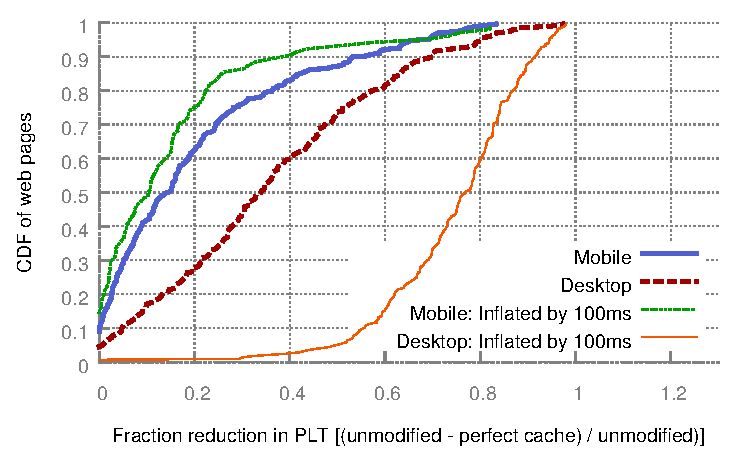
\includegraphics[width=3in]{../graphs/percent_plt_reduction/percent_reduction_linear_inflated.pdf}
%    \caption[]{\label{fig:inflated_delays}In networks with high latency, caching has a negligible effect on mobile PLTs, but a significant benefit for desktop PLTs.}
    % Just remove the first sentence of the caption?
%\end{figure}



\section{Conclusion}
\label{sec:conclusion}
We have presented an experimental apparatus for examining the effects of caching on mobile page load time.
Using this apparatus, we demonstrate that mobile page load time is not significantly reduced by caching, contrary to common wisdom.
We go further to show that resource constraints, specifically the CPU, appears to be the main difference between caching's effect on desktop versus mobile.
Content providers may want to reconsider where they focus their optimization efforts, especially as mobile traffic begins to outpace its desktop counterpart.

In future work we plan to measure the critical path on mobile devices, experiment with other web page load time metrics, further levels of caching, and inflating the original network delays to better emulate mobile devices in congested network environments. 

Going forward, mobile devices are becoming increasingly powerful and the bottleneck resources will shift. At what point will web caching have a larger benefit for mobile?  

%\subsection{Future Work}
%There is still space to explore these findings. Using other metrics such as above-the-fold PLT and SpeedIndex may provide deeper insight into the reasoning behind limited mobile PLT reduction. Similarly, examining changes in the critical path with a tool such as WProf would provide valuable insight (WProf does not currently have a mobile tool). 

%It is also worth experimenting with varying levels of caching, namely 22\% and  32\% as in the Google NSDI paper~\cite{flywheel} to see if such incremental changes to mobile PLT are observed. \jamshed{Remove if done.}

%Finally, it is worth adding fixed delays to network responses in order to better emulate mobile and congested networks.


%\renewcommand{\baselinestretch}{0.9843}

%\appendix
\section{Model Derivation}
\label{sec:appendix}

% Not sure where this content goes yet... but here's an explanation....
Here we derive the page load time performance model stated in~\ref{subsec:model}. We
develop a continuous probability model (i.e., we assume that the size of all
objects sums to 1.0), since we are not aiming for a high degree of accuracy,
and since discrete models are more unwieldly.

%This model is useful for those determining how many resources (money, effort, time, etc) to put into developing an effective cache (such as a CDN).
%That is, with our model, one can estimate the return on investment that is gained by caching.

We introduce one term in addition to those in~\ref{subsec:model}:

\noindent--Let $K$ denote the fraction of objects that are on the critical path.

In our derivation we override the terms $X$ and $K$ to also denote random
variables: the event that a given object is cached and the event that a given
object is on the critical path, respectively.

We make two simplifying assumptions in deriving our model. First, we assume that the probability that an
object is present in the cache is independent of the probability that the
object is on the critical path.\footnote{
This first assumption is likely overly conservative; Figures 11a and 11b of the
WProf paper seem to indicate that objects on the critical path may have lower
probability of being cacheable than other objects~\cite{wang2013demystifying}.}
Second, we assume that the critical path does not change as we vary the cache hit
ratio. That is, we treat $K$ as a constant.

We categorize all objects on the critical path into two distinct groups.
The first category is the fraction of all objects on the critical path that are cached (these
will incur 0 network delay, assuming that the cache is colocated with the
browser):

\begin{align*}
Pr(X|K) & =  Pr(X) & \text{[since $X$ and $K$ are independent]} \\
& = X &
\end{align*}

The second category is the fraction of all items on the critical path that are not cached (these will incur their original network delay):

\begin{align*}
Pr(1-X | K) & = Pr(1-X) & \text{[since $X$ and $K$ are independent]} \\
& = 1-X &
\end{align*}

At a given cache hit ratio $X$, the expected value of the total network delay
on the critical path is (assuming that a cached item incurs zero network delay):
\begin{align*}
E_N[X] & = Pr(X|K) \cdot 0 + Pr(1-X|K) \cdot N \\
& = (1 - X) \cdot N
\end{align*}

Thus, the total expected PLT given a hit ratio $X$ is:
\begin{align*}
E_{PLT}[X] & = C + E_N[X] - f(C,N,X) \\
& = C + (1 - X) \cdot N - f(C,N,X)
\end{align*}

% TODO(cs): To generalize this model to a case where the cache is located far away from
% the browser... we could introduce a non-zero fetch cost associated with
% cached items.


%\theendnotes

\end{document}
